\chapter{Technical Foundations and Possible Models}
\label{ch:foundations}

The literature review identified five research design requirements: target validity, representation suitability, incremental fusion value, input reliability, and methodological validity. This chapter builds the technical foundations needed to explore these requirements, focusing on the representation and fusion mechanisms related to SQ1–SQ3.

The architecture family studied here includes modality-specific representations, prediction models, and ways to combine their information. These parts can be tested separately or put together in different experimental setups. This modular approach lets us explore specific representation and fusion options without assuming one setup works for all industrial monitoring tasks.

The next sections cover the common prediction setup, visual and temporal representations, reference predictors, and both static and adaptive fusion methods. When needed, the first published architectures are set apart from the specific components used in this thesis. Details about dataset preparation, fitting steps, and assessment methods are given in Chapter~\ref{ch:methodology} and the related empirical chapters.

\section{Common Mathematical Notation and Prediction Formulation}

Industrial monitoring tasks can be formulated as regression or classification problems depending on the target of interest. Regression estimates a continuous quantity, such as a derived condition indicator, whereas binary classification estimates whether an observation belongs to a specified outcome class.

An individual prediction unit may represent a gear experiment run, robotic action, milling interval, or manipulation episode. Each prediction unit belongs to a dependence group representing a relevant acquisition or operational grouping.

The principal multimodal classification architectures consider visual and machine-sensor observations. Investigations involving several sensor groups use an equivalent formulation with an extended set of input branches.

Each prediction unit is associated with its available observations, modality availability indicators, optional process or measured-quality context, and prediction target.

For binary classification, the positive outcome is defined separately for each empirical study. In REASSEMBLE, ViFailback, and HANDOVER, the positive outcome represents failure. In MSM, it represents abnormal cutting under the adopted target definition.

A modality-specific encoder transforms the available observations into a representation. This representation may consist of engineered statistical features or learned embeddings. A prediction head subsequently transforms the representation into a scalar regression estimate or classification score.

For classification, a sigmoid function maps a real-valued score into the interval between zero and one. Although this procedure produces a bounded probability estimate, it does not automatically establish that the resulting predictions are calibrated.

The logit transformation, \(\ell(p)=\log[p/(1-p)]\), converts a probability into its corresponding log-odds. Numerical implementations require appropriate clipping at the probability boundaries to avoid undefined logarithms.

Fusion can occur at different points in this prediction process. Feature-level fusion combines modality representations before the final prediction head, while prediction-level fusion combines modality-specific scores or probabilities. The distinction determines the information available to the fusion system and the relationships it can learn.

\section{Visual Representations}

Industrial monitoring frequently involves limited independently acquired samples relative to the capacity of modern visual architectures. Pretrained convolutional representations therefore provide a reasonable candidate for extracting reusable spatial information without fitting an entire visual encoder from the available target-specific observations.

The success of transferred intermediate CNN features in industrial inspection supports investigating such representations, although their suitability for completed-action classification requires separate evaluation \parencite{Roth2022Towards}.

\subsection{Convolutional Feature Extraction and Spatial Pooling}

A convolutional encoder transforms an input image into hierarchical feature maps. Earlier layers typically represent local visual patterns, while deeper layers can encode more abstract spatial and semantic information.

Each feature map consists of multiple channels with corresponding spatial dimensions. Global average pooling converts each feature channel into a scalar by averaging its spatial activations.

The pooled representations obtained at different scales are concatenated to form a frame-level descriptor. For an observation containing several selected frames, a complete-window representation can subsequently be obtained through temporal averaging.

This procedure produces a condensed representation whose dimensionality remains independent of the starting spatial feature-map resolution and the number of sampled frames.

Spatial pooling retains information about the average activation of each feature channel but removes explicit spatial coordinates and local correspondence. Temporal averaging adds another restriction because the resulting representation is independent of frame order.

The representation can therefore exploit differences in visual content across an observation window without explicitly modelling the temporal sequence in which those differences occur.

A convolutional reference remains important when Transformer-based components motivate the architectural investigation. The Vision Transformer study shows that the relative effectiveness of convolutional and attention-based architectures depends on the scale of available pretraining data, with convolutional inductive biases remaining valuable in smaller-data settings \parencite{P010}.

Video Swin introduces local spatiotemporal attention and shifted windows as an alternative for processing video sequences. Its computational resource requirements depend on the evaluated temporal clips and spatial crops \parencite{P013}.

These architectures provide alternative mechanisms for retaining visual information. Their published results motivate comparative investigation rather than establishing greater performance than a frozen convolutional representation under the sample availability and fitting budgets of this thesis.

\subsection{RT-DETR Architecture and Component Roles}

RT-DETR is a real-time object detection architecture that combines a convolutional backbone, a hybrid encoder for multi-scale feature interaction, and a query-based detection decoder \parencite{Zhao2024RTDETR}.

The convolutional backbone extracts hierarchical spatial features from the input image. The hybrid encoder supports within-scale and cross-scale interaction between visual features. The Transformer-based decoder uses object queries to produce object-level representations, while the detection heads generate object classifications and bounding-box predictions.

The scientific rationale for investigating the backbone concerns the availability of pretrained multiscale spatial features. The additional hybrid encoder provides a separate candidate for investigating whether further spatial feature interaction improves the downstream representation.

The object detection performance reported by \textcite{Zhao2024RTDETR} motivates the investigation of these components but does not establish their predictive suitability for industrial action outcomes.

\subsection{Backbone Extraction Versus Hybrid-Encoder or Full-Detector Execution}

The principal REASSEMBLE visual representation uses the ResNet18-vd convolutional backbone contained in the pretrained RT-DETR-R18vd checkpoint, identified as \nolinkurl{PekingU/rtdetr_r18vd}.

After loading the pretrained detector, the implementation selects the convolutional backbone and freezes its parameters. Three multiscale feature maps are extracted and spatially averaged, producing an 896-dimensional representation for each image.

Sixteen frames are sampled from each completed action. Their frame-level representations are averaged to form a single 896-dimensional action descriptor. A separately trained binary classification head then predicts the recorded action outcome.

The hybrid Transformer encoder, query-based detection decoder, and bounding-box prediction heads are bypassed in this core experiment.

The later CNN-versus-spatial-encoder comparisons investigate an additional visual representation in which the backbone and hybrid encoder are both involved. These comparisons constitute separate architectural configurations with their own feature dimensions and fitting budgets.

The PHM visual-regression investigation uses a different extraction procedure. It invokes the Ultralytics prediction path with a frozen RT-DETR-L checkpoint and collects three intermediate multiscale feature maps through registered hooks. Spatial pooling produces a 768-dimensional visual representation.

The recorded implementation additionally includes extraction latency as a numerical covariate, resulting in a 769-dimensional input to the regression head. Consequently, the PHM visual head receives both image-derived information and a timing-related variable.

\noindent\textit{Internal implementation evidence.} \EvidenceRef{E064}{}, \EvidenceRef{E065}{}, \EvidenceRef{E033}{}.

\subsection{Frame Sampling, Feature Aggregation, and Temporal Modelling}

Fixed frame sampling provides a reproducible number of observations for each prediction unit. It limits computational variation between clips of different lengths and allows the subsequent prediction head to receive a fixed-dimensional representation.

However, a fixed sampling procedure may overlook brief events, including short contact changes or transient visual evidence of failure. The suitability of the sampling strategy therefore depends on the duration and visibility of the phenomenon associated with the prediction target.

Alternative aggregation procedures can retain additional temporal structure. Boundary pooling restricts the representation to frames occurring within a selected part of an operation, while temporal bins preserve coarse information about the progression of the observation window. Recurrent neural networks and temporal Transformers provide more flexible mechanisms for learning order-dependent relationships.

TimeSformer separates spatial and temporal attention and reports advantages for its divided attention mechanism over the other tested attention configurations on Kinetics-400 and Something-Something V2 \parencite[Table~1]{P034}. This provides a scientific motivation for investigating temporal organization, although it does not directly establish the suitability of a particular boundary-pooling rule.

The principal REASSEMBLE representation uses sixteen deterministically sampled hand-camera frames. Images are resized to a resolution of \(640 \times 640\) pixels, and their numerical values are divided by 255. No additional ImageNet mean and standard-deviation normalization is applied in the recorded core procedure.

These preprocessing choices describe the executed implementation rather than a universal preprocessing requirement for RT-DETR.

The comparison between whole-action averaging and boundary-aware pooling investigates whether restricting the aggregation interval preserves more useful information for completed-action classification. Because the prediction target is associated with the completed action, the use of observations close to its conclusion does not establish early-warning capability.

The corresponding empirical comparisons are presented in Chapter~6.

\subsection{Frozen Extraction and Visual Fine-Tuning}

Pretrained visual representations can be adapted to a target task at different levels. Frozen extraction retains the parameters learned during pretraining and fits only a downstream prediction head. Partial fine-tuning modifies selected encoder components, while full-backbone fine-tuning updates the complete selected visual encoder.

Frozen extraction reduces the number of trainable parameters and allows extracted representations to be cached. This can make repeated model fitting within grouped evaluation procedures computationally feasible.

Fine-tuning provides the opportunity to adapt visual features to the appearance and operational characteristics of the target dataset. Its effectiveness nevertheless depends on supervision, sample availability, and optimization conditions.

Comparisons between frozen and adapted representations require consideration of normalization-layer states, augmentation, learning rates, early stopping, batch sizes, and optimization steps. The number of training epochs alone does not establish that two configurations received equivalent optimization opportunities.

Generic COCO initialization, REASSEMBLE-supervised donor initialization, and target-domain adaptation represent distinct interventions.

A generic frozen encoder transfers representations learned during external pretraining. A donor encoder introduces information learned through supervision on the source task. Target-domain adaptation modifies the encoder using observations and labels from the new task.

These distinctions are relevant to the ViFailback experiments, which separately investigate frozen generic representations, transferred REASSEMBLE representations, and the completed portion of target-backbone adaptation.

The existence of extracted or cached features establishes that the corresponding extraction stage occurred. It does not independently establish that downstream classification, fusion fitting, or assessment was completed.

\section{Sensor and Time-Series Representations}

Machine-sensor observations describe physical quantities and operational states through sequential measurements. Their usefulness depends on how the available channels relate to the prediction target and how their temporal information is represented.

This thesis investigates two principal representation families: engineered statistical summaries and learned patch-based temporal representations.

The two families impose different restrictions on the information available to a predictor. Statistical summaries retain selected properties of an observation window while discarding much of its original temporal order. Learned sequence representations offer greater flexibility in modelling ordered observations but introduce additional fitting requirements.

Their comparison therefore addresses whether explicit temporal modelling retains useful information beyond compact summaries and whether the two representations provide complementary predictive value.

\subsection{Statistical and Signal-Derived Features}

Conventional engineered features remain scientifically relevant in industrial applications. For example, classical local geometric representations have demonstrated competitive performance in industrial 3D anomaly detection, supporting the need to retain strong engineered references when evaluating learned representations \parencite{Horwitz2023Back}.

In REASSEMBLE, ten statistical features are calculated for each of the 22 progress-resampled sensor channels. These features include the mean, standard deviation, median, minimum, maximum, lower quartile, upper quartile, range, root-mean-square amplitude, and linear progress slope.

The mean and median describe the central measurement level, while the standard deviation and quartiles characterize its distribution. The minimum, maximum, and range describe the observed extrema and their separation. The root-mean-square amplitude represents measurement magnitude, and the linear progress slope describes coarse directional change across the action.

The resulting feature vector contains 220 features. These features retain information concerning location, spread, magnitude, and coarse trend while discarding most detailed temporal ordering.

Such features provide a deliberate restriction on the information available to the prediction model. They can represent operating states without requiring a high-capacity sequence encoder to be fitted using limited independently acquired observations.

The available sensor channels include force, torque, gripper-related measurements, joint effort, and joint velocity. Their statistical representation tests whether compact descriptions of the completed action provide sufficient information for the prediction target.

Spectral representations provide another approach to summarizing sequential measurements. Their interpretation depends on the physical sampling rate and preprocessing interval. A sequence resampled according to action progress is not equivalent to a uniformly sampled physical vibration signal. Frequency-domain interpretations must therefore respect the acquisition and resampling procedures.

MSM uses a separate representation derived from its controller measurements, while PHM uses minute-level sensor and process-context features. These representations are defined according to their respective measurement systems and prediction targets rather than treated as interchangeable feature vectors.

\subsection{PatchTST Architecture}

PatchTST introduces a patch-based approach to time-series representation learning. Instead of treating every individual timestamp as a separate Transformer token, the architecture divides a sequence into local subsequences called patches \parencite{Nie2023PatchTST}.

Each patch is transformed into a learned embedding. The resulting embedding sequence is processed by Transformer layers that can model relationships between different temporal positions.

The original PatchTST architecture incorporates channel-independent processing with shared model parameters across channels. This structure allows temporal relationships within individual channels to be represented without requiring a separate independently parameterized Transformer for every measurement channel.

Patching provides two potential advantages. First, local subsequences retain information about neighbouring measurements within each patch. Second, representing a sequence through patches reduces the number of tokens processed by the attention mechanism relative to a representation in which every timestamp is treated separately.

The original work indicates the relevance of this approach for time-series forecasting \parencite{Nie2023PatchTST}. Its use in this thesis concerns a different prediction problem: supervised condition estimation or outcome classification.

The investigated PatchTST implementations therefore adapt the underlying architectural principles to their respective targets. They are initialized from scratch rather than transferring pretrained PatchTST weights.

This distinction is necessary because evaluating a scratch-trained Transformer-based encoder does not establish the effectiveness of pretrained time-series representation transfer.

\subsection{Patching, Sequence Length, Padding, and Aggregation}

The patch width determines how many successive observations are included within each token, while the stride determines the displacement between consecutive patches.

Padding and masking procedures can change the number of generated patches and the observations available to the representation. Consequently, the theoretical patch count must be distinguished from the number of tokens actually processed by a particular implementation.

After temporal encoding, a pooling or aggregation procedure transforms the patch-level representations into a fixed-dimensional descriptor suitable for downstream prediction.

The core REASSEMBLE implementation resamples each action to 512 progress positions across 22 sensor channels. The scratch-trained PatchTST classifier uses a patch width of 32, a stride of 16, a hidden representation width of 32, two Transformer layers, four attention heads, and a feed-forward width of 64.

Figure~\ref{fig:sensor-patch-tokens} shows how two overlapping patches of one channel become separate tokens.

\begin{figure}[H]
\centering
\caption{From Overlapping Sensor Patches to Tokens. One schematic REASSEMBLE sensor channel is shown from an action resampled to 512 progress positions across 22 channels. Patches 1--32 and 17--48 share positions 17--32; their starts are 16 positions apart. The trace illustrates the construction rather than an observed recording.}
\label{fig:sensor-patch-tokens}
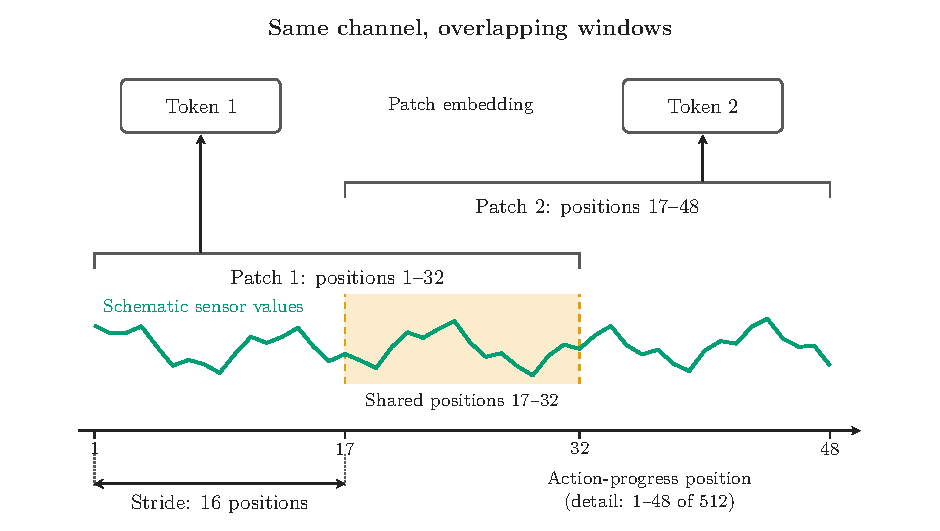
\includegraphics[width=\linewidth]{figures/review_explanatory_20261126/sensor_patch_tokens.pdf}
\end{figure}

Under an unpadded regular grid, these sequence and patch dimensions produce 31 patches. The executed token count additionally depends on the model’s padding configuration.

The implementation averages the encoded patch representations and concatenates the channel representations before applying a projection into a 128-dimensional feature space.

Internal model scaling is disabled because standardization is performed externally. An observed-value mask is also supplied to the model. However, the presence of this argument alone does not establish how every missing observation affects attention and aggregation. Its interpretation depends on the executed masking operations.

The PHM implementation uses a separate custom patch-based regression encoder. Its default patch width is 16, with stride 8, and its input consists of variable-length minute-level sequences.

Patch validity is determined by the presence of at least one valid temporal position within the patch, followed by masked aggregation. The implementation raises a concern regarding the dependence of its patch grid on batch sequence length. The numerical effect of this behaviour on the historical experimental results remains unmeasured.

The PHM architecture additionally predicts sorted profiles through positive increments. Sorting removes tooth identity from the predicted representation, restricting the interpretation of these outputs to ordered profiles rather than tooth-specific localization.

Alternative time-series representation methods provide further context for the investigated encoder. TS2Vec uses a dilated convolutional architecture with hierarchical contrastive learning. Its reported backbone ablation illustrates that replacing a convolutional representation with a Transformer does not necessarily improve downstream classification \parencite{P012}.

MOMENT instead investigates pretrained time-series Transformers through masked reconstruction across datasets. Its downstream evaluations distinguish the use of pretrained representations from supervised classifier fitting \parencite{P018}.

These approaches motivate further investigation of learned temporal representations. Nevertheless, comparisons with the scratch-trained PatchTST branches must retain differences in pretraining, available supervision, and fitting budgets.

\noindent\textit{Internal implementation evidence.} \EvidenceRef{E031}{}, \EvidenceRef{E065}{}.

Table~\ref{tab:ch3-representations} summarises the representation paths and their fitted predictors.

\begin{table}[htbp]
\caption{Executed Representation Paths in PHM and REASSEMBLE}\label{tab:ch3-representations}
\centering\small\setstretch{1}
\begin{tabularx}{\linewidth}{@{}P{0.24\linewidth}YY@{}}
\toprule
\textbf{Component} & \textbf{Input and representation} & \textbf{Fitted predictor or use} \\
\midrule
PHM scalar-image branch & RT-DETR-L prediction path with three hooked maps. Pooling yields 768 image features, and extraction latency adds one covariate. & Scalar regression head receives 769 inputs. \\
PHM temporal branch & Variable-length minute features with a custom PatchTST-style encoder. Default patch length 16 and stride 8. & Scratch-trained regressor with a scalar output or an optional sorted-profile head. \\
REASSEMBLE visual branch & Frozen ResNet18-vd backbone in RT-DETR-R18vd, 16 frames, and an 896-dimensional pooled action descriptor. & Fitted binary head. The core path bypasses the detector's hybrid encoder, decoder, and prediction heads. \\
REASSEMBLE sensor statistics & Ten summaries per channel across 22 channels yield 220 features. & Training-side scaling and logistic regression. Supplies the sensor probabilities used by the core stacker and gates. \\
REASSEMBLE temporal branch & \(512 \times 22\) progress-aligned input. Patch length 32 and stride 16, followed by pooling and a 128-dimensional projection. & Scratch-trained PatchTST and binary head. Evaluated separately as a sensor-only comparator in the core fusion study. \\
\bottomrule
\end{tabularx}
\displaynote{See Appendix~C for the implementation details and Appendix~\ref{app:reproducibility} for the executed component map.}
\end{table}

\subsection{Representation Learning Versus Direct Prediction}

A learned encoder can be used for different purposes within a prediction architecture. It may provide a reusable representation for a downstream model, directly predict a target, or supply features to a multimodal fusion mechanism.

A generic pretrained encoder can generate fixed features without using the labels associated with the target assessment population. Such representations can be cached if their preprocessing and sample identities remain consistent.

In contrast, an encoder trained using target-specific supervision becomes part of the fitted prediction system. Its training must therefore respect the evaluation partitions associated with the downstream task.

The distinction also applies to the statistical-feature and PatchTST comparison. Both representations originate from the same physical sensor observations. Any improvement obtained by combining them concerns representation complementarity rather than the contribution of an additional independently acquired modality.

\section{Prediction Models and Reference Baselines}

A suitable comparison requires more than a weak baseline. The reference should represent a credible alternative under the available data and fitting conditions, enabling the contribution of additional information or model complexity to be investigated.

\subsection{Constant and Simple Reference Predictors}

For regression, the training mean minimizes squared error within the training population. The training median minimizes absolute error.

The principal PHM comparison retains the training mean as its recorded historical reference. The mathematical suitability of the median for absolute error does not imply that a median-based comparison was executed.

Context-only predictors provide another useful reference. Process identity, action duration, or time index may contain predictive information even when the principal sensor observations are unavailable.

For example, action identity may be associated with different failure frequencies, while a condition proxy may vary with experiment progression. A context-only reference can therefore help assess whether an apparent improvement requires additional physical measurements or can be partly explained by contextual predictability.

\subsection{Linear and Logistic Models}

Ridge regression estimates a continuous target by minimizing squared prediction error together with a squared coefficient penalty.

For binary classification, logistic regression represents the probability of the positive outcome by applying a sigmoid transformation to a linear combination of input features and a fitted intercept.

The model is generally fitted using a cross-entropy objective, with regularization controlling the magnitude of its coefficients.

Its performance depends on preprocessing, feature standardization, regularization, class weighting, and solver configuration.

In the principal REASSEMBLE statistical-sensor comparison, the regularization parameter is selected from three candidate values: 0.1, 1, and 10. The selection is performed within the permitted training partitions.

The core F2 stacker uses a fixed regularization parameter of 1. This value belongs to the recorded implementation configuration and is not described as the outcome of a separate hyperparameter search.

\subsection{Neural Classification and Regression Heads}

A compact feed-forward head may first transform the input representation through an affine layer followed by a nonlinear activation function. Additional regularization, including dropout during training, can be applied before the final scalar prediction layer.

In the core REASSEMBLE experiments, the visual and PatchTST classification heads are fitted using class-weighted binary cross-entropy. The original context-conditioned gates instead use unweighted binary cross-entropy.

The core visual prediction head contains 114,945 trainable parameters in addition to the frozen convolutional backbone.

The corresponding PatchTST sensor module contains 109,505 trainable parameters across its encoder, projection, and classification components. Of these, 90,369 belong to the projection and classifier.

These counts describe the fitted capacity of the respective configurations. They do not independently establish equivalent computational cost or optimization difficulty.

\subsection{Other Models Relevant to Retained Experiments}

Histogram gradient boosting provides a nonlinear conventional alternative to regularized linear prediction.

This model family is particularly relevant to the external dataset studies because outperforming a logistic sensor component does not necessarily establish superiority over a stronger conventional sensor predictor.

The ViFailback histogram-gradient-boosting comparison uses its recorded validation-based candidate-selection procedure. The corresponding MSM result belongs to its separate controller-feature protocol.

The detailed configurations of the additional prediction models are documented in Appendix~C.

Table~\ref{tab:ch3-reference-predictors} shows the role of each reference in the comparisons.

\begin{table}[htbp]
\caption{Reference Predictors and the Comparisons They Support}\label{tab:ch3-reference-predictors}
\centering\small\setstretch{1}
\begin{tabularx}{\linewidth}{@{}P{0.24\linewidth}YY@{}}
\toprule
\textbf{Reference} & \textbf{Predictor input or fitting rule} & \textbf{Use in the thesis} \\
\midrule
Constant regression & Training mean. The training median minimizes absolute loss in the training data. & PHM uses the training mean as its recorded reference. \\
Class prevalence and context & Training prevalence, or available context such as action type. & Separates a simple reference or context-based predictability from the value of physical observations. \\
Regularized linear models & Ridge regression for continuous targets and logistic regression for binary outcomes. & Provides a fitted reference with compact inputs, including the REASSEMBLE statistical sensor predictor. \\
Single-modality neural heads & A fitted head on visual or temporal features. & Provides branch-level references for testing the value of fusion. \\
Histogram gradient boosting & An additive tree model on binned numerical features. & Provides a nonlinear sensor comparison in the external studies. Fitting and selection follow each dataset's protocol. \\
\bottomrule
\end{tabularx}
\displaynote{Appendix~C describes the recorded model configurations.}
\end{table}

\section{Fusion Mechanisms}

The investigated mechanisms include feature concatenation, uniform probability averaging, logistic stacking, context-conditioned scalar gating, and subsequent adaptive extensions.

These mechanisms differ in the information supplied to the fusion stage, the number and constraints of trainable parameters, and whether the relative contribution of each branch can vary between observations.

Their comparison addresses R3 and R4 by examining whether additional information improves prediction and whether adaptation provides benefits beyond simpler integration mechanisms.

\subsection{Feature Concatenation}

The visual and sensor representations are concatenated into a common feature vector. Separate projection functions may first transform the representations into suitable feature spaces before the combined representation is processed by a prediction head.

Feature concatenation provides access to the information retained within the contributing representations. A nonlinear downstream head may learn interactions between individual features originating from different input branches.

However, increasing the dimensionality of the combined representation can also increase the fitted model capacity. A comparison with a unimodal model may therefore change both the available information and the number of trainable parameters.

The retained PHM \texttt{fused\_all\_three} implementation combines representations from process-context, RMS, and condition-indicator encoders before a scalar regression head.

Although its implementation class is named \texttt{LateFusionRegressor}, its executed computation combines embeddings rather than separate predicted probabilities. It is therefore classified here as feature-level fusion.

This PHM configuration combines sensor-derived groups rather than representing a camera–sensor inference architecture. Equal final embedding dimensions also do not imply equivalent total encoder capacity.

\noindent\textit{Internal implementation evidence.} \EvidenceRef{E004}{Section~12.4}.

\subsection{Uniform Prediction Averaging}

The core F1 baseline assigns equal importance to the visual and sensor probability estimates by calculating their arithmetic mean.

The integration rule contains no fitted combination parameters, although its component predictors and their calibration procedures are fitted using the respective training observations.

This makes F1 a useful comparator for investigating whether learning a more flexible integration mechanism produces additional predictive value.

The averaging of probabilities is distinct from averaging logits and subsequently applying a sigmoid. These procedures generally produce different probability estimates.

Furthermore, averaging two calibrated probability estimates does not automatically establish that the combined probability remains calibrated.

When one input is unavailable, the averaging rule requires an additional policy specifying whether the surviving prediction is returned, the weights are renormalized, or the system abstains.

\subsection{Logistic Stacking}

Stacked generalization provides a methodological foundation for learning a second-stage prediction model from the outputs of first-stage predictors. \textcite{Ting1999Issues} investigate the construction of this learning problem using cross-validated predictions, allowing the second-stage model to learn from outputs obtained for observations excluded from the corresponding first-stage fitting.

The original publication evaluates a different combination model from the logistic stacker investigated in this thesis. Its methodological contribution motivates the construction of a second-stage prediction problem rather than establishing the suitability of the exact F2 configuration.

The core F2 mechanism combines the calibrated visual and sensor probabilities using a logistic prediction model. Its fitted parameters consist of an intercept and two branch coefficients. The weighted combination of the branch probabilities and the intercept is transformed through a sigmoid function.

\begin{equation}
 p_{\mathrm{F2}}=\sigmoid(b+\alpha_v p_v+\alpha_s p_s).
 \label{eq:f2}
\end{equation}

Here, \(p_v\) and \(p_s\) are the visual and sensor probabilities, \(b\) is the intercept, and \(\alpha_v\) and \(\alpha_s\) are their fitted coefficients.

Unlike a convex weighted average, the branch coefficients are not required to be positive or sum to one. The stacker can therefore learn unequal contributions from its inputs while adjusting the resulting prediction through its intercept and logistic transformation.

Its three-parameter structure provides a compact mechanism for investigating whether a fitted combination improves on equal probability averaging.

The coefficients must not be interpreted as normalized modality importance scores or causal estimates of the information contributed by each physical observation.

The retained core REASSEMBLE procedure constructs branch out-of-fold predictions that exclude the recording associated with each predicted training row. Its outer assessment recordings are excluded from model fitting.

However, the internal validation of the stacker reuses an out-of-fold prediction bank constructed within the outer training population. This introduces a deeper training-side dependency that restricts claims of strict nesting. Chapter~\ref{ch:methodology} and Chapter~6 establish the corresponding assessment boundaries.

Model selection using evaluation data can introduce optimistic estimates of selected predictive performance \parencite{P004}. Leakage prevention must therefore consider the actual preprocessing, fitting, calibration, and prediction-bank dependencies rather than relying on the use of an out-of-fold label alone \parencite{P017}.

\subsection{Context-Conditioned Scalar Gating}

A gating network receives available process or quality information \(u\) and produces an allocation score \(q_m(u)\) for each modality \(m\). The modality weights are calculated through masked softmax normalization, which excludes unavailable branches and normalizes the contributions of the remaining inputs.

The normalization is defined when at least one modality remains available. If both modalities are absent, the normalization becomes undefined and the original implementation rejects the input.

The weights are nonnegative and sum to one across the available modalities.

\begin{equation}
 w_m(u,a)=\frac{a_m\exp(q_m(u))}{\sum_j a_j\exp(q_j(u))},\qquad
 p_G=\sigmoid\left(\sum_m w_m(u,a)\ell(p_m)\right).
 \label{eq:gate}
\end{equation}

Here, \(a_m\in\{0,1\}\) indicates modality availability and \(p_m\) is its branch probability.

The principal REASSEMBLE investigation considers three types of conditioning. The action-context gate receives action-related process information and has an input width of six. The quality-context gate receives measured-quality descriptors and has an input width of 38. The combined gate incorporates both forms of context and has an input width of 42. These dimensions include the two modality availability indicators.

These gates combine scalar modality predictions rather than intermediate image regions or sensor tokens.

Gated Multimodal Units combine hidden representations through learned conditional allocation \parencite{P006}, while multimodal attention bottlenecks exchange information through shared intermediate tokens \parencite{Nagrani2021MBT}. These architectures provide relevant precedents for context-dependent integration but are not mathematically equivalent to the scalar gates implemented in this thesis.

The original gates use logit inputs without a free final intercept or a separate post-gate calibration stage. F2, in contrast, receives probabilities and includes a fitted intercept with unconstrained branch coefficients.

A predictive performance difference between these mechanisms may therefore reflect differences in their input transformations, coefficient constraints, intercepts, or fitting procedures as well as differences in adaptive allocation.

The gate’s weights provide descriptive information about how the fitted model allocates its predictions. They do not independently identify physical failure causes or establish that the selected allocation accurately reflects the reliability of a modality.

\subsection{Quality-Conditioned Interactions and Adaptive Extensions}

The theoretical investigation of dynamic fusion by \textcite{Zhang2023QMF} establishes conditions relating uncertainty, unimodal losses, and generalization bounds under which adaptive weighting may provide benefits.

These conditions motivate the use of context-dependent information but do not establish that an arbitrary measured-quality descriptor provides an accurate estimate of predictive reliability.

The subsequent anchored adaptive extension investigates whether context-dependent adjustment can improve a previously fitted static fusion model.

Rather than replacing the F2 coefficients with normalized softmax weights, the anchored mechanism retains its fitted intercept and branch coefficients and learns multiplicative adjustments to those coefficients.

\begin{equation}
 p_A=\sigmoid\left[b+\sum_m\alpha_m\{1+\tanh(h_m(u))\}p_m\right].
 \label{eq:anchored}
\end{equation}

The adjustment network produces the branch-specific output \(h_m(u)\).

The final adjustment layer is initialized to zero, causing the initial adaptive model to reproduce its fitted F2 anchor.

For finite adjustment-function outputs, the multiplicative adjustment lies between zero and two. However, the underlying branch coefficients remain unconstrained and can be signed. The resulting coefficients are therefore not normalized reliability weights.

A constant-adjustment control investigates whether observation-dependent variation provides additional predictive value beyond another fixed parameterization.

A subsequent quality-interaction study compares alternative prediction heads under matched augmentation exposure. This constitutes a separate controlled investigation rather than another component of the original scalar-gate experiment.

Measured-quality descriptors may summarize observable coverage, signal properties, or other characteristics of an input. Model confidence instead describes the prediction model’s own output. Calibrated probability quality concerns the agreement between predicted probabilities and observed outcomes.

These quantities are related but not interchangeable.

A quality-aware fusion mechanism must therefore establish through empirical comparison whether its available descriptors help identify situations in which a modality becomes less informative or produces misleading predictions.

Calibration can deteriorate under distribution shift, and uncertainty-estimation methods do not consistently dominate across all evaluated conditions \parencite{P008}.

Consequently, clean-data calibration, changes in fusion weights, and improved robustness under degradation represent distinct empirical findings.

\subsection{Missing-Modality Routing and Fallback}

When one branch is unavailable and the other remains accessible, the masked normalization of the original context-conditioned gate assigns a weight of one to the surviving branch.

The original REASSEMBLE robustness evaluator explicitly returns the surviving branch probability and applies that branch’s threshold. If both branches are unavailable, the system rejects the input.

If different fusion mechanisms return the same surviving branch prediction, their performance under known absence is identical for those fixed branch outputs. Such a comparison evaluates the fallback policy rather than demonstrating a benefit from learned adaptive weighting.

Training-time modality dropout may influence the behaviour of a model when the available inputs change. Nevertheless, training exposure to missing observations must be distinguished from an empirically measured improvement under a specified absence condition.

ModDrop introduces training mechanisms that expose multimodal models to unavailable inputs \parencite{P005}. EmbraceNet investigates stochastic feature selection together with modality-availability information \parencite{P007}. Missing-modality Transformer studies further examine architectures trained and evaluated under incomplete-input conditions \parencite{P016}.

Figure~\ref{fig:fusion-interfaces} shows the prediction interfaces of the core stacker and context-conditioned gates.

\begin{figure}[htbp]
\caption{Inputs to the REASSEMBLE Stacker and Context-Conditioned Gates}\label{fig:fusion-interfaces}
\centering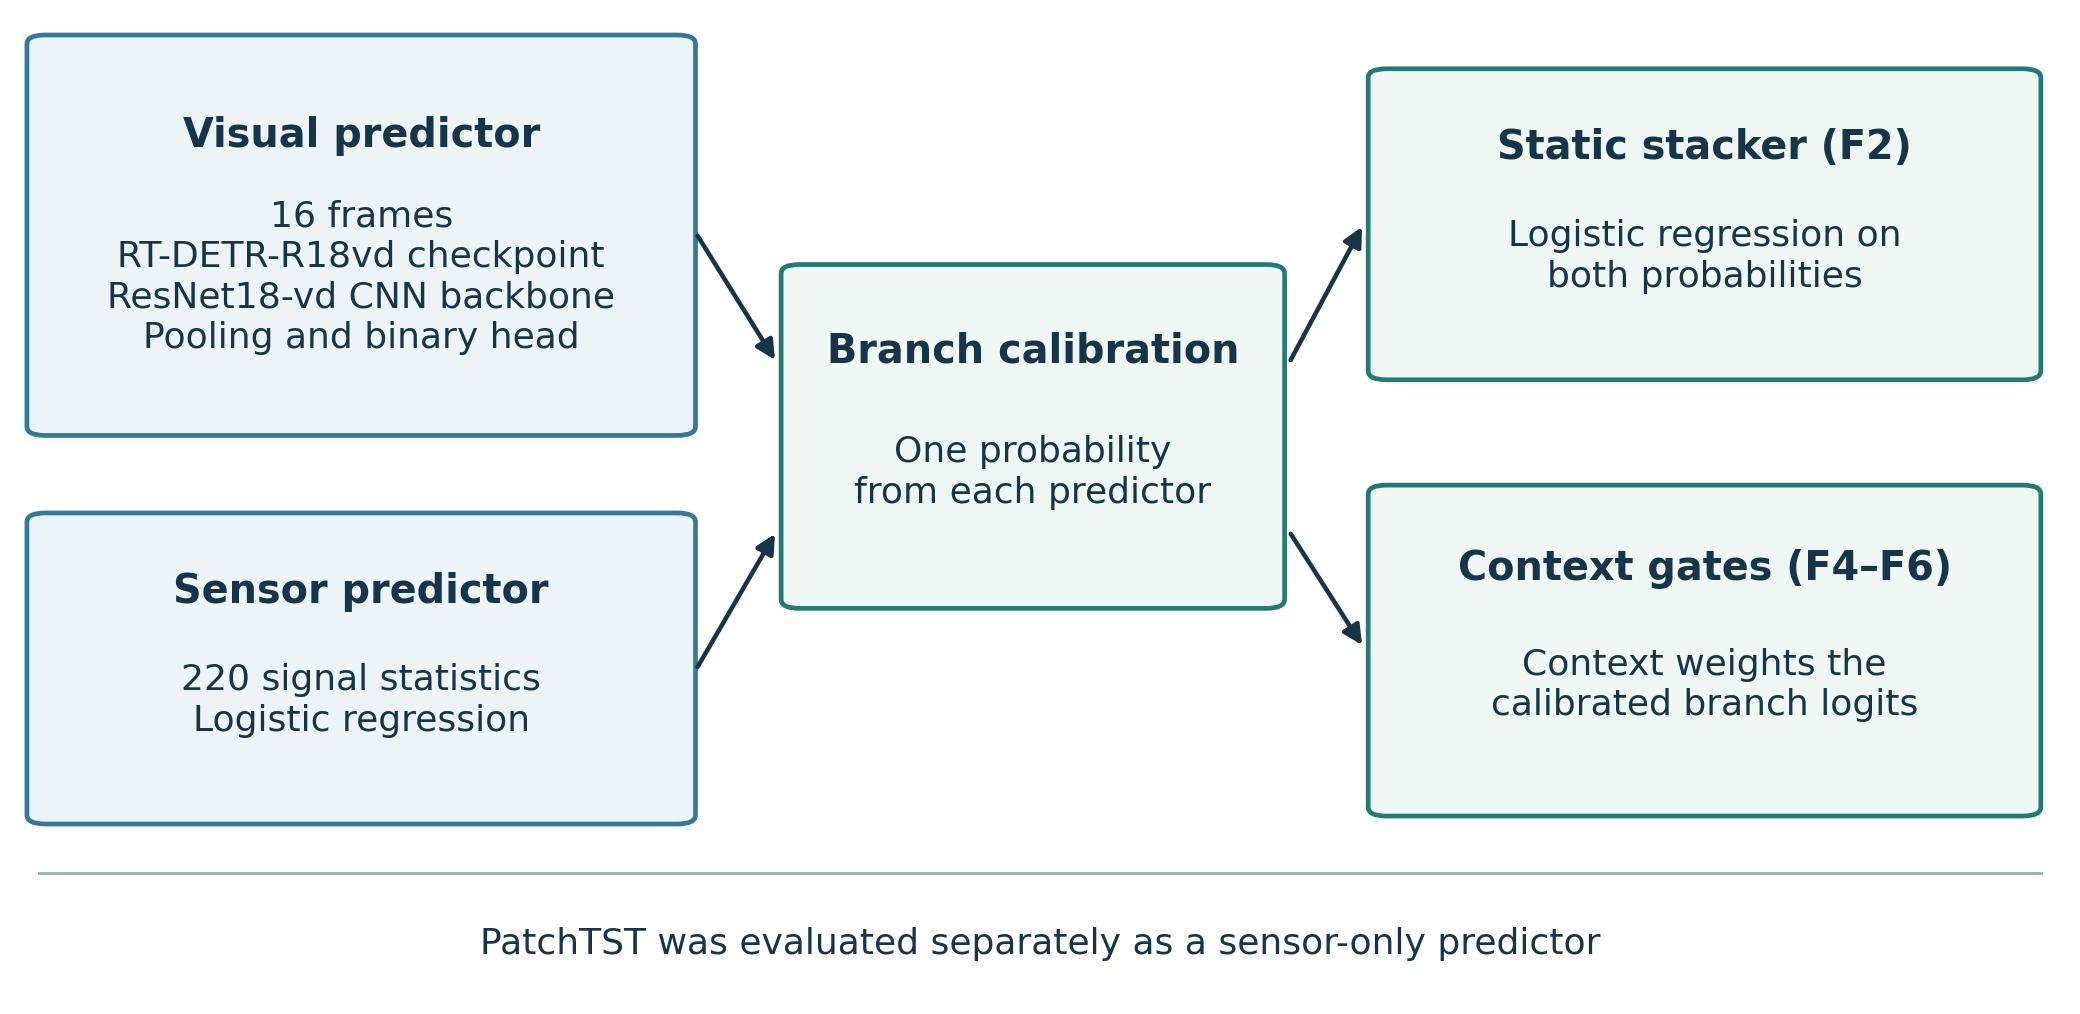
\includegraphics[width=\linewidth]{figures/fusion_interfaces}
\displaynote{The stacker and all three gates used the statistical sensor predictor. PatchTST was evaluated separately as a sensor-only comparator in the core experiment. Each branch supplied a calibrated probability. The gates converted those probabilities to logits before weighting them.}
\end{figure}

Table~\ref{tab:ch3-fusion-interfaces} collects the distinctions between their inputs and combination rules.

\begin{table}[htbp]
\caption{Inputs and Combination Rules for the Investigated Fusion Mechanisms}\label{tab:ch3-fusion-interfaces}
\centering\small\setstretch{1}
\begin{tabularx}{\linewidth}{@{}P{0.24\linewidth}YY@{}}
\toprule
\textbf{Mechanism} & \textbf{Input to fusion} & \textbf{Combination rule} \\
\midrule
Feature concatenation & Modality embeddings or PHM sensor-group embeddings. & Concatenated features feed a fitted prediction head. \\
Uniform averaging (F1) & Calibrated branch probabilities. & Fixed arithmetic mean. \\
Logistic stacking (F2) & Calibrated branch probabilities. & A fitted intercept and a weighted sum of branch probabilities enter a sigmoid. \\
Context gates (F4--F6) & Branch logits and action context, quality context, or both, with availability indicators. & Masked softmax provides observation-dependent weights for the branch logits. \\
Anchored adjustment & Branch probabilities and context descriptors. & Context adjusts the fitted F2 coefficients multiplicatively while retaining the intercept. \\
\bottomrule
\end{tabularx}
\displaynote{The core REASSEMBLE stacker and all three original context gates use the statistical sensor predictor. PatchTST is a separate sensor-only comparator in that experiment.}
\end{table}

\section{Component Selection Criteria and Implementation Mapping}

The original REASSEMBLE protocol established a bounded comparison consisting of a pretrained convolutional backbone with a fitted prediction head, compact statistical sensor representations, and a scratch-trained patch-based temporal encoder.

The protocol explicitly recognized that the limited neural fitting budget could not exclude improvements from longer training.

These records establish the historical starting configuration. They do not establish that the exact visual checkpoint or temporal encoder settings were selected through an exhaustive comparative search over alternative architectures.

The later selection of statistical sensor features for the principal fusion investigation followed the initial experimental results. This decision therefore forms part of the exploratory model-selection history.

The scientific justification of the investigated components can be distinguished from their documented historical selection.

These representation choices address R2 by examining different restrictions on retained information and different fitting requirements.

Feature concatenation, equal probability averaging, and logistic stacking address R3 through alternative integration mechanisms. Their comparison investigates whether combining representations or predictions provides incremental value and whether a fitted combination improves on a simpler fixed rule.

Context-conditioned gates and anchored adaptive extensions introduce the possibility that the usefulness of information varies between observations. These mechanisms address R3 and R4 by examining whether adaptive combinations improve predictive performance and reliability. Missing-input routing additionally establishes a defined system response under declared modality absence.

The original research question also considers acoustic representations. The Audio Spectrogram Transformer provides a scientifically relevant pretrained candidate for such observations, with its reported performance depending on the evaluated acoustic task and model configuration \parencite{P011}.

The REASSEMBLE correspondence and label-leakage concerns prevented the admission of an acoustic prediction branch. The architectural investigation therefore retains audio as a literature-supported candidate rather than a completed predictive component.

The implementation map in Appendix~\ref{app:reproducibility} and the configuration records in Appendix~C document the executed prediction paths. These records distinguish the candidate architectures from the components that were trained and evaluated.

The technical mechanisms described in this chapter are not all components of one jointly evaluated final system. Individually favourable representation, pooling, and adaptive-fusion configurations remain separate experimental interventions unless their combination was explicitly assessed.

Chapter~\ref{ch:methodology} establishes the shared research methodology through which these components are investigated. It connects their technical properties to target validity, modality correspondence, assessment independence, predictive performance, uncertainty, and reliability conditions associated with requirements R1–R5.

\noindent\textit{Internal implementation evidence.} \EvidenceRef{E112}{}, \EvidenceRef{E114}{}, \EvidenceRef{E110}{}.
